\chapter{Ice reservoirs}

\cleanchapterquote{Glaciers are the secret of life in these otherwise lifeless deserts. But now, they are
	melting away at an alarming rate.}{Sonam Wangchuk}{(Ramon Magsaysay awardee,\\ Inventor of ice stupas)}


\section{Introduction}

Mountains contribute disproportionately to global water resources, considering their geographical extent.
Due to their buffering capacity, for instance by supplying glacial meltwater during the hot and dry season,
they provide a relatively constant water supply to downstream areas. Worldwide, the vast majority of glaciers
are losing mass \citep{zempGlobalGlacierMass2019a}, snow melt dynamics are being perturbed
\citep{mukhopadhyayReevaluationSnowmeltGlacial2015, hammondGlobalSnowZone2018}, and precipitation and
evapotranspiration patterns are shifting; all these leading to future vulnerability of mountain water availability
\citep{lutzConsistentIncreaseHigh2014}. These changes are believed to be largely and negatively
impacting agriculture across many different mountainous regions \citep{ipccCrossChapterPaperMountains2022}.

These issues are particularly pronounced in arid and semiarid regions, where it is estimated that between 50\%
and 90\% of freshwater resources originate from mountain catchments
\citep{mukhopadhyayReevaluationSnowmeltGlacial2015, messerliMountainsWorldVulnerable2004}. As a consequence,
mountain communities have developed some nature-based water storage solutions and farming practices, namely,
bofedales \citep{monge-salazarEcohydrologyEcosystemServices2022}, amunas
\citep{ochoa-tocachiPotentialContributionsPreInca2019}, rock glacier oasis \citep{pandeyRockGlacierOasis2022},
and \ac{AIRs} \citep{wangchukIceStupaCompetition2020} to cope with climate-change-induced water stress.

\citet{immerzeelImportanceVulnerabilityWorld2020} quantify the importance of these mountain regions by
classifying river basins as \ac{WTUs}. Globally, a total of 78 \ac{WTUs} are home to more than 250 million
people. Among these, the most important WTUs lie in \ac{HMA}, where communities are increasingly relying on
\ac{AIRs} for climate change adaptation (Fig. \ref{fig:WTUs_AIRs}). 

\ac{AIR} building is a long tradition, with records dating back more than 50 years
\citep{nusserSociohydrologyArtificialGlaciers2019}. \ac{AIRs} capture water in the autumn and winter, allowing
it to freeze and holding it until spring, when it melts and flows down to the fields
\citep{ipccChapterHighMountain2019, vinceGlacierMan2009, clouseLadakhArtificialGlaciers2017,
nusserSociohydrologyArtificialGlaciers2019}. In this way, they retain an otherwise unused portion of annual
flow and facilitate its use, supplementing the decreased flow during the following spring (Fig.
\ref{fig:irrigation_cycles}). Over the past decade, several \ac{AIRs} have been built to supplement the
irrigation water supply of mountain villages in India \citep{wangchukIceStupaCompetition2020,
palmerStoringFrozenWater2022, aggarwalAdaptationClimateChange2021}, Pakistan
\citep{awazproductionIceStupaArtificial2022}, Kyrgyzstan \citep{bbcnewsBrightArtificialGlacier2020}, Nepal, and
Chile \citep{reutersConservationistsChileAim2021}. In total, more than 500 farmers have constructed \ac{AIRs} across
30 villages in the Alps, Andes, and \ac{HMA} (Fig. \ref{fig:WTUs_AIRs}).

\begin{figure}[htb]
	\centering
	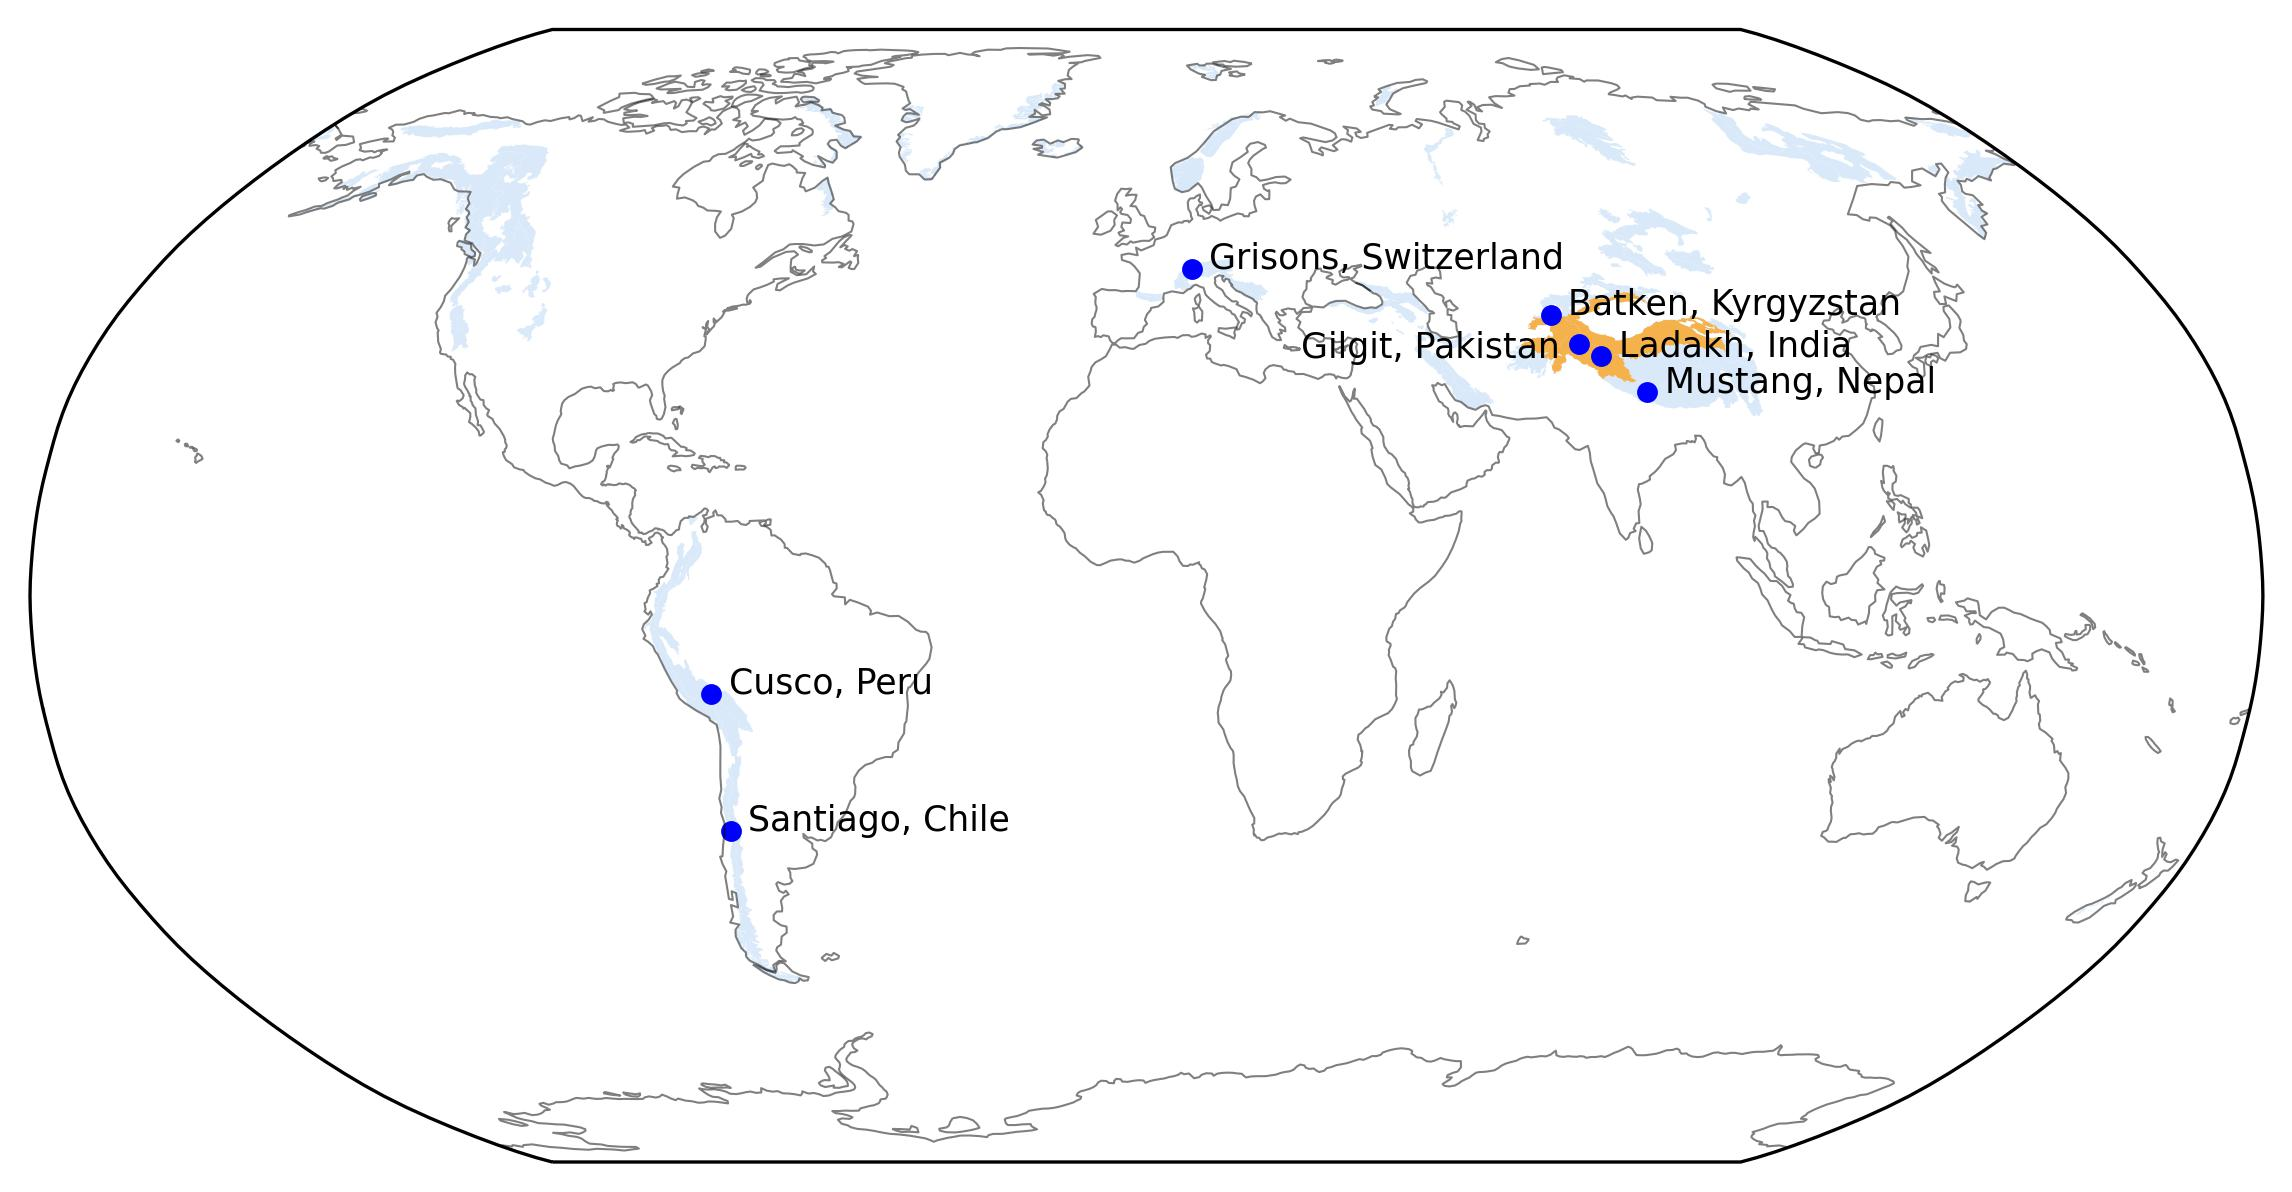
\includegraphics[width=\textwidth]{figs/WTUs_AIRs.jpg}

	\caption{ Global distribution of water tower units (light blue) based on
		\citet{immerzeelImportanceVulnerabilityWorld2020}. The most important \ac{WTUs} (orange) are also situated where most 
		AIR construction sites  are located (dark blue). }

	\label{fig:WTUs_AIRs}
\end{figure}

\begin{figure}[htb] \centering 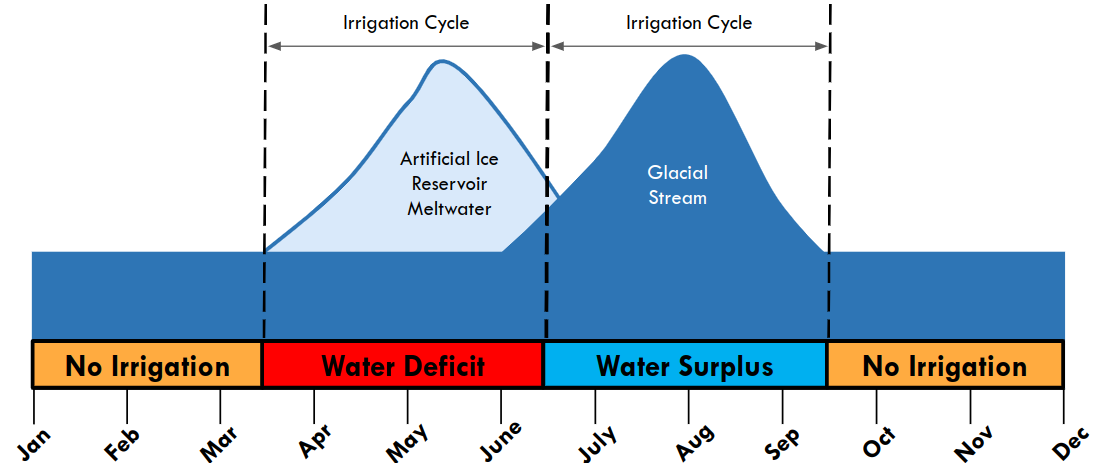
\includegraphics[width=\textwidth]{figs/irrigation_cycles.png}
	\caption{Seasonal variation in availability of irrigation water in Ladakh, India. The graph highlights the
		crucial role of \ac{AIRs} in bridging the gap in water availability. Adapted from
		\citet{nusserLocalKnowledgeGlobal2016}.} \label{fig:irrigation_cycles} \end{figure}


Despite this widespread adoption, only a few publications have examined the role of \ac{AIRs} in the water resource
management of these regions. Notably, none of these prior reports have investigated \ac{AIRs} outside Ladakh.
Moreover, the available estimates of water storage capacity of \ac{AIRs} in Ladakh vary widely
\citep{norphelSnowWaterHarvesting2015, baglaArtificialGlaciersHelp1998}.

Quantifying the water storage capacity of \ac{AIRs} is not straightforward, since the processes by which
\ac{AIRs} are formed are complex. These processes are controlled by local topography, meteorology, and the
construction strategies used. Modelling approaches to quantify these processes exist on glacier surfaces, but
they are not readily applicable for \ac{AIRs} due to their limited size and their comparatively more variable surface
area. Therefore, conventional modelling approaches used in glaciology need to be adapted to capture the
spatiotemporal scale of \ac{AIR} surface processes. Furthermore, these modelling approaches need to be validated and
calibrated with comprehensive data from field measurements.

A spirit of improvisation guides the construction of \ac{AIRs} \citep{clouseLadakhArtificialGlaciers2017}.
Depending on the local topography and on how water is supplied, \ac{AIRs} can form as flat sheets or vertical
cones, and are therefore referred to as ice terraces or ice stupas, respectively (Fig. \ref{fig:AIRforms}). This
results in \ac{AIRs} exhibiting significant volume variations despite experiencing similar
meteorological conditions. For example, in Ladakh, India, ice terraces have attained volumes up to 30 times
larger than ice stupas \citep{nusserSociohydrologyArtificialGlaciers2019}. However, the processes driving these
differences can only be understood if the complete design methodology behind each construction is available.

\begin{figure}[t]
	\centering
	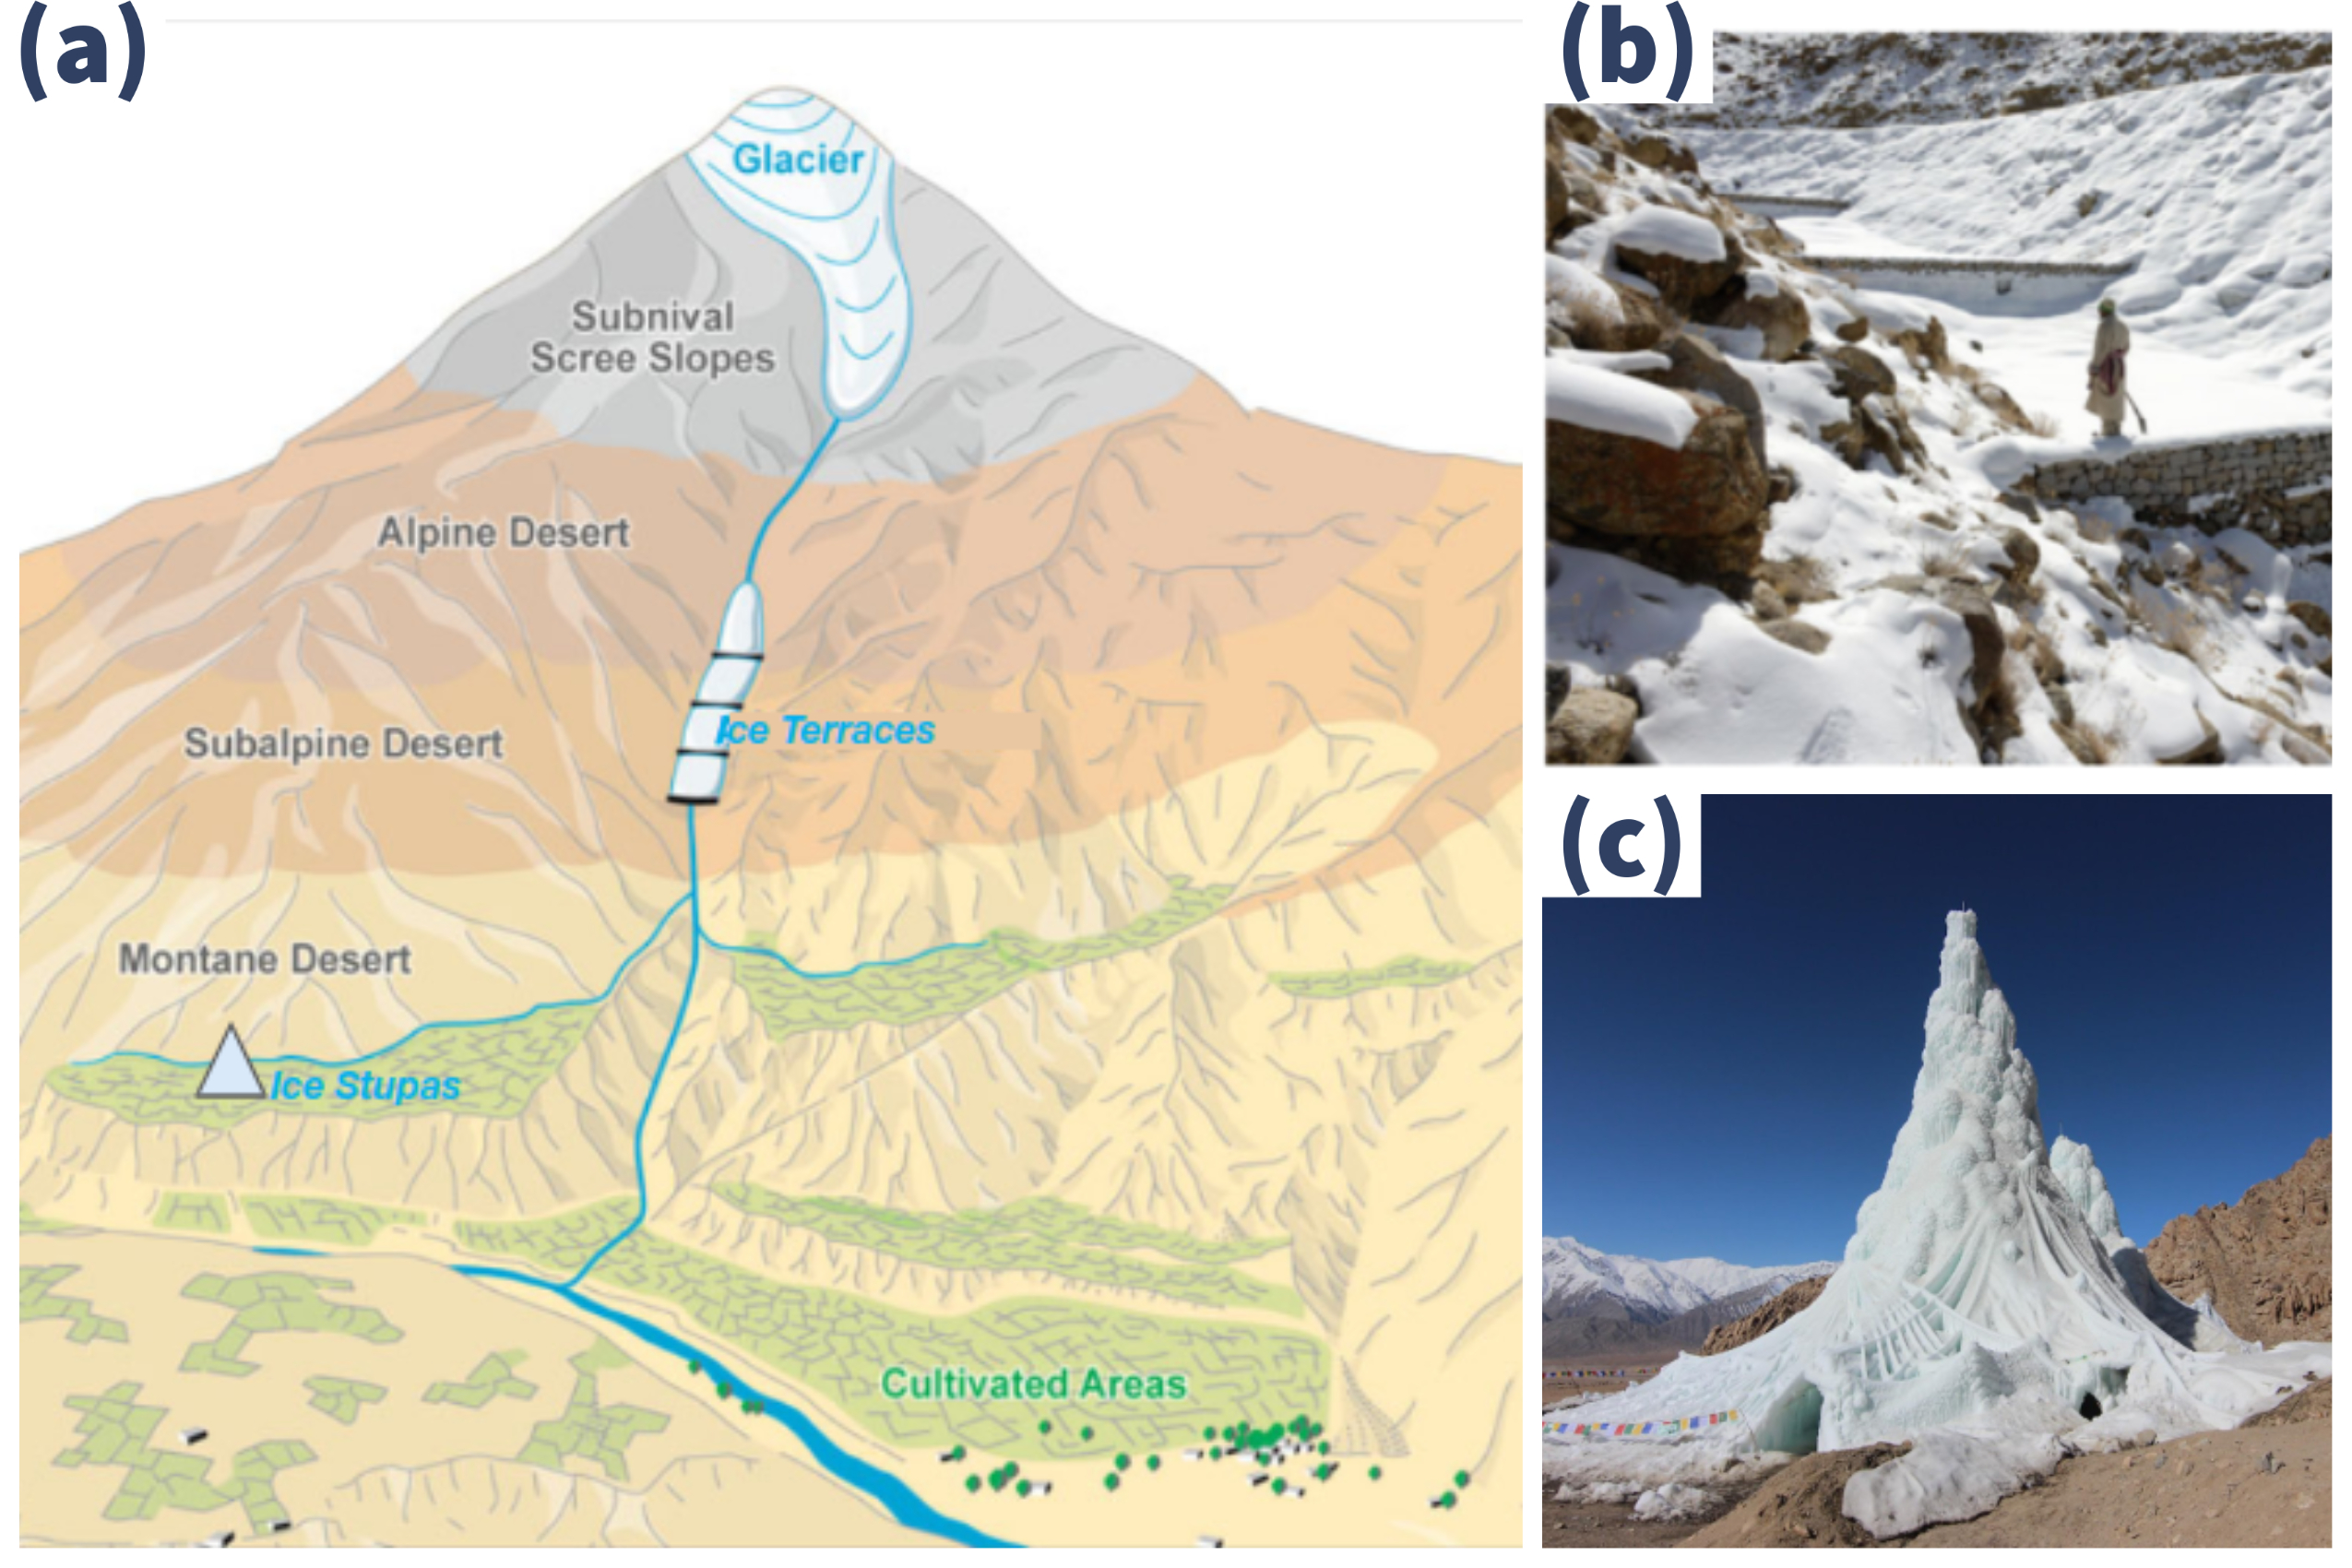
\includegraphics[width=\textwidth]{figs/AIR_forms.jpg}

	\caption{ (a) Schematic overview of the position of artificial ice reservoirs. These constructions are located at
		altitudes between the glaciers and the irrigation networks in the cultivated areas. (b) Ice terraces at 3900
		$m$ \ac{a.s.l.}, located above the village of Nang, Ladakh. The cascade is composed of a series of loose masonry walls
		ranging in height from 2 to 3 $m$, which facilitate the freezing of water. (c) Ice stupas at 3600 m, located
		above the village of Phyang, Ladakh. They are constructed using fountain systems. Adapted from \citet{nusserLocalKnowledgeGlobal2016}. }

	\label{fig:AIRforms}
\end{figure}

This thesis aims to fulfill the abovementioned requirements by providing a new set of \ac{AIR}-specific volume and area
measurements via drone flights, along with meteorological data recorded during the construction period. All these
datasets are obtained from construction strategies that involve fountain systems. These systems are quantified
via \textit{in situ} observations of the fountain characteristics and discharge rate measurements. First, one- and two-dimensional models are formulated, calibrated, and validated with the procured \ac{AIR} datasets. Then,
these models are used as tools to propose a construction strategy that can produce \ac{AIRs} efficiently and
effortlessly. While this thesis reviews published research, substantial additional knowledge is held by the
farming communities building these structures since the mid-1800s.


\section{Nomenclature and classification}

The term "artificial glacier" is commonly used by local farmers to refer to \ac{AIRs}
\citep{norphelArtificialGlacierHigh2009}. However, many believe this term can be misleading
\citep{nusserSociohydrologyArtificialGlaciers2019}. By definition, all glaciers, including the smallest ones,
are bodies of sedimentary ice built by progressive snow compaction and firnification that flow
downhill under the influence of gravity \citep{benndouglasGlaciersGlaciation2014}. Hence, because of their
genesis and composition, \ac{AIRs} differ from glaciers. Human-made ice structures typically have a lifetime in
the order of months and a size a million times smaller than natural glaciers. The term \ac{AIRs} is used in this thesis to
distinguish the man-made ice structures described above from the natural ones.

However, when classified in terms of size and survival duration, \ac{AIRs} exhibit similar characteristics to
very small glaciers. The glossary of glacier mass balance and related terms by
\citet{cogleyGlossaryGlacierMass2010} defines very small glaciers or glacierets as follows:

\begin{thesis_quotation}
	A very small glacier, typically less than 0.25 $km^2$ in extent, with no marked flow pattern
	visible at the surface. To qualify as a glacieret, an ice body must persist for at least two consecutive
	years. Glacierets can be of any shape, and usually occupy sheltered parts of the landscape. Windborne snow and
	avalanches can be dominant contributors to the accumulation of glacierets.
\end{thesis_quotation}

This rather broad definition of glacierets or very small glaciers may be best suited to describe \ac{AIRs}, since
they present areas as large as 0.15 $km^2$ \citep{nusserSociohydrologyArtificialGlaciers2019} and
have been observed to last beyond a year.

As noted above, \ac{AIR} construction strategies are usually inspired by a spirit of improvisation, which challenges
their classification. However, construction strategies using fountain systems have been found to form
conical \ac{AIRs}, while others form flat sheets of ice. \ac{AIRs} using fountain systems are called
"ice stupas", and those not using them are called "ice terraces"; this terminology denotes the resulting shape of the
respective \ac{AIRs}.

\section{Research aim and outline}

The preceding sections show that many of the small-scale surface processes that occur on \ac{AIRs} are complex
and not well understood at present and that their interplay remains uncertain. These need to be unraveled to be able to better predict the
water storage potential of \ac{AIRs} and to improve their water storage efficiency under different climate conditions and with different
construction methodologies. Therefore, the main objective of the present thesis is:

\begin{thesis_quotation}

  \textbf{To increase the understanding of volume dynamics of artificial ice reservoirs and to
  provide tools that reduce their water losses and maintenance requirements.}

\end{thesis_quotation}

Data on \ac{AIRs} are scarce, which is the reason for many of the unknowns and uncertainties around the dynamics
of these ice structures. This thesis therefore has a strong focus on the implementation of measurement campaigns
using drones and \ac{AWS} to achieve its main objective. The thesis touches on two different topics that
address the following specific research questions:

\begin{enumerate}

  \item \textit{What is the influence of construction location and fountain characteristics on ice stupa volume
    evolution?}

Three process-based models for ice stupas were designed to answer the first research question. Since \textit{in situ}
    measurements were required to run this model, measurement campaigns were executed in Switzerland and India
    during the past four winters (2018/19, 2019/20, 2020/21, and 2021/22). These datasets provided the necessary
    input, calibration, and validation data to model the evolution of ice stupas and study their sensitivity to
    meteorological conditions and fountain characteristics. Description of the study sites and overview of these
    models are presented in the \textit{Science} chapter. Results from their application are presented in the
    \textit{Habitat} chapter.

  \item \textit{How can ice stupa fountain systems be engineered to reduce water losses and maintenance
    efforts?}

To answer this question, a new construction strategy was developed using an automation system. The automation
    hardware incorporated the models developed to regulate fountain discharge rate. The description of the
    automation system and its advantages over manual construction strategies are presented in the
    \textit{Technology} chapter.

\end{enumerate}

In addition to the chapters mentioned above, the \textit{Religion} chapter illustrates the origin of ice harvesting
solutions among mythologies and religious practices; in the \textit{Heritage} chapter, the main findings
presented in this thesis are placed into a broader perspective through some recommendations; and the
\textit{Papers} chapter lays out the peer-reviewed work supporting this thesis.


